\begin{center}
\begin{tikzpicture}[x=1cm,y=1cm]
%\pgfresetboundingbox
\draw[use as bounding box, anchor = north west,draw,dashed,gray] (-5.5,-3.25) rectangle (5.5,3.25);
\clip (-5.5,-3.25) rectangle (5.5,3.25);
\only<6->{\node[anchor =north west] (text) at (-5.25,3.25){\begin{minipage}{10.0cm}Let's return to our previous example:
		\end{minipage}};}
\only<1-5>{\node[anchor =north west] (text) at (-5.25,3.25){\begin{minipage}{10.0cm}
Adapting model complexity to fit the problem is necessary. However, it is not obvious how to do this is a constrolled way.\\
Hence, we need a way prevent over-fitting that is applicable to many different types of model -- \textbf{Regularization}.\\
\visible<2->{We instead choose to minimize:
\begin{small}
\begin{align*}
\mathcal{L}'(y,f(x,w)) &=\mathcal{L}(y,f(x,W)) + \lambda R(W) \\
 \visible<3->{(\textrm{Tiknohov/Ridge})&=\frac{1}{n}\left\Vert y - f(x,W)\right\Vert_2^2 +{\only<4->{\color{red}} \lambda \left\Vert W \right\Vert_2^{2}}}
\end{align*}
\end{small}}
\visible<4->{We choose to {\color{red}penalize terms with large weights}, i.e. complicated functions}.
\visible<5>{\begin{itemize}
\item This makes empirical errors worse.
\item This \textit{can} improve generalization/excess risk.
\end{itemize}}
\end{minipage}};}
\visible<6->{\node (figure) at (-2.75,0){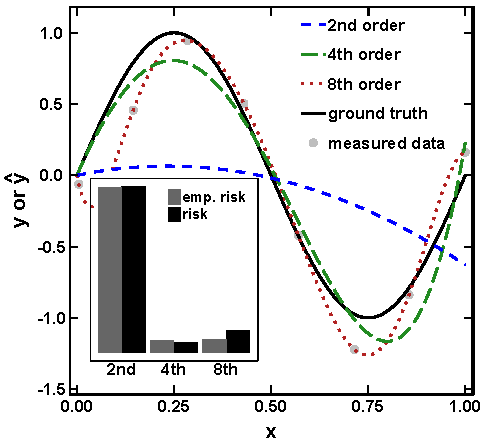
\includegraphics[width=5cm]{satistical_learning/figures/comp_6.pdf}};}
\visible<7->{\node (figure) at (2.75,0){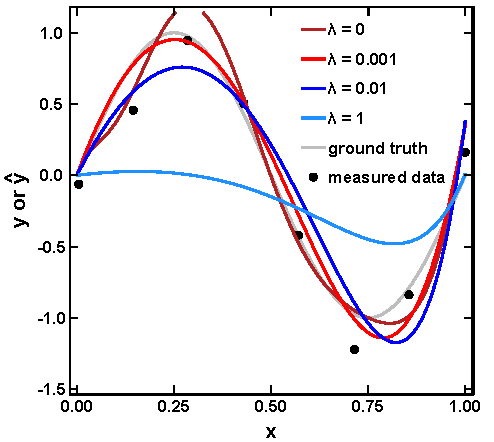
\includegraphics[width=5cm]{satistical_learning/figures/lam_2.pdf}};}
\visible<8->{\node (figure) at (2.75,0){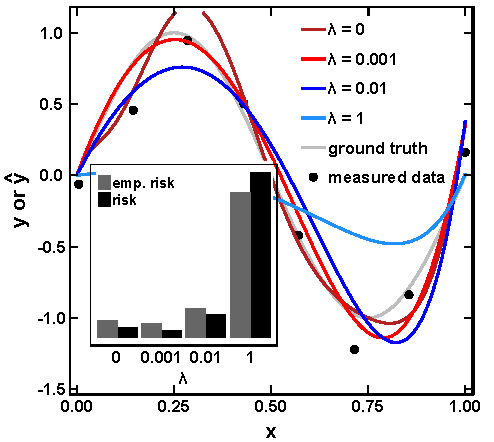
\includegraphics[width=5cm]{satistical_learning/figures/lam_3.pdf}};}
\only<6->{\node[anchor =north west] (text) at (-5.25,-2.75){\begin{minipage}{10.0cm}Remember: larger $\lambda=$ simpler, flatter model. \end{minipage}};}
\end{tikzpicture}
\end{center}